\documentclass[12pt]{article}
\usepackage{hyperref}
\usepackage{amsmath, amssymb, amsfonts}
\usepackage[margin=1.2cm]{geometry}
\usepackage{xcolor}
\usepackage{graphicx}
\usepackage{enumitem}
\parindent 0pt
\newcommand{\lb}{\\$\left|\rightarrow\right.$}
\newcommand{\enter}{\\\textcolor{white}{1}}
\ExplSyntaxOn
\NewDocumentCommand{\bo}{m}
 {
   \bold_commas:n { #1 }
 }
\cs_new:Npn \bold_commas:n #1
 {
   \seq_set_split:Nnn \l_tmpa_seq { , } { #1 }
   \seq_map_indexed_function:NN \l_tmpa_seq \__bold_commas_aux:nn
 }
\cs_new:Npn \__bold_commas_aux:nn #1 #2
 {
   \textbf{#2}
   \int_compare:nNnTF { #1 } < { \seq_count:N \l_tmpa_seq }
     { , }
     { }
 }
\ExplSyntaxOff

\title{Data Mining (CT72502 / CT725)\\[0.4em]\large Detailed PYQ 69--82}
\author{}
\date{\today}

\begin{document}
\maketitle
\vspace{6cm}
\textbf{Notes}
\begin{itemize}[noitemsep]
  \item Questions from Tribhuvan University, IOE (2069--2082 BS), sorted by the CT72502 syllabus.
  \item Regular exam = \bo{bold}, Back / New Back exam = regular font.
  \item Data Mining is a \emph{single common paper} for both BEX and BCT (Elective I / Elective II), so there is no separate programme axis --- no \texttt{monospace} style is used in this document.
  \item So: \bo{80 Bh} = Regular, 81 Ba = Back.
  \item Months: Ba = Baishakh, Asa = Ashad, Shr = Shrawan, Bh = Bhadra, Ash = Ashwin, Ka = Kartik, Ch = Chaitra. Note \textbf{Asa (Ashad) and Ash (Ashwin) are different months}: 70 Asa and 70 Ch are the two 2070 papers.
  \item Keywords: (I) = Importance/Need/Significance, (+) = Advantage, (-) = Disadvantage, +Fig = Figure/Diagram, +Eg = Example, Vs = Compare/Differentiate.
  \item Papers covered (23): \bo{82 Bh}, \bo{81 Bh}, 81 Ba, \bo{80 Bh}, 80 Ba, \bo{79 Bh}, 79 Ba, \bo{78 Bh}, \bo{76 Ch}, 76 Ash, \bo{75 Ch}, 75 Ash, \bo{74 Ch}, 74 Ash, \bo{73 Ch}, 73 Shr, \bo{72 Ch}, 72 Ka, \bo{71 Ch}, 71 Shr, 70 Asa, \bo{70 Ch}, \bo{69 Ch}. There was no exam in 2077, and no 2082 Baishakh paper.
  \item \bo{71 Ch} and 71 Shr print no per-question marks (``All questions carry equal marks'', 80 marks total).
  \item Course code by year: \bo{69 Ch} prints \emph{no} course code (just ``Data Mining (Elective I)''), \bo{70 Ch} prints CT725, and every other paper prints CT72502.
  \item Programme by year: BEX/BCT throughout, except \bo{82 Bh}, which prints \textbf{BCT, BEI}, and \bo{81 Bh}, which misprints \textbf{BCT, BCT}.
\end{itemize}
\pagebreak
\tableofcontents
\pagebreak

%=======================================================================
\section{Introduction}
\begin{center}(2 Hours)\end{center}

  \subsection{Data Mining Origin}
    \begin{enumerate}[topsep=0pt, noitemsep]
      \item What is data mining? Explain the process of data mining. \hfill [2+3] (74 Ash)
        \lb What is data mining? Explain all the steps of knowledge discovery. \hfill [2+6] (\bo{72 Ch})
        \lb What is Data Mining? What are the steps involved in knowledge discovery process? \hfill [1+5] (\bo{79 Bh})
        \lb What is Data mining? Explain the steps of KDD process briefly. \hfill [2+5] (81 Ba)
        \lb What is a data mining? Explain general steps in brief. \hfill [4] (72 Ka)
        \lb What is a Data Mining? Explain its application. \hfill [10] (\bo{71 Ch})
        \lb What is data mining? Describe the steps involved in data mining. \hfill [2+6] (\bo{82 Bh})
        \lb Describe the process of knowledge discovery in databases. Explain the specific challenges that motivated the development of data mining. \hfill [3+3] (79 Ba)

      \item ``The world is data rich but information is poor''. Justify with your own words. \hfill [8] (73 Shr)
        \lb ``Data mining turns a large collection of data into knowledge''. Justify your answer with suitable example. \hfill [6] (\bo{81 Bh})
    \end{enumerate}

  \subsection{Data Mining \& Data Warehousing basics}
    \begin{enumerate}[topsep=0pt, noitemsep]
      \item What is data warehousing? Explain with example where data warehouses are used. \hfill [2+4] (80 Ba)
        \lb Write key features of data warehouse. Explain each steps of knowledge discovery data mining process with a suitable example. \hfill [2+5] (\bo{80 Bh})
        \lb Explain Data Warehouse architecture with its analytical processing. \hfill [8] (\bo{75 Ch})

      \item What are the fundamental differences between Data Mining and Data Warehousing? Describe the steps of KDD for data mining. \hfill [3+7] (76 Ash)
        \lb How is data warehouse different from a database? How are they similar? \hfill [2+2] (75 Ash)
        \lb How is data warehouse different from RDBMS? Also list the similarities. \hfill [2+2] (\bo{73 Ch})

      \item Explain how data mining system can be integrated with database/data warehouse system. Explain Data mining process with diagram. \hfill [4+2] (\bo{78 Bh})

      \item What is data warehouse and data mart? Describe Snowflake scheme with example. \hfill [2+4] (\bo{74 Ch})

      \item Write short notes on: Data ware house and Data mart. \hfill [15] (\bo{70 Ch}) [--] (71 Shr)
        \lb Write short notes on: Data ware house. \hfill [5] (70 Asa)
        \lb Write short notes on: Datamart. \hfill [5] (\bo{69 Ch})
    \end{enumerate}

\pagebreak
%=======================================================================
\section{Data Preprocessing}
\begin{center}(6 Hours)\end{center}

  \subsection{Data Types and Attributes}
    \begin{enumerate}[topsep=0pt, noitemsep]
      \item What is data mining? Explain different data types of attributes in a dataset. \hfill [10] (71 Shr)
        \lb What are the different data types? Explain with examples. \hfill [5] (\bo{69 Ch})

      \item What are nominal and ordinal attributes? Discuss how to handle missing data and noisy data during data cleaning process. \hfill [6] (79 Ba)

      \item How data in most real application becomes Asymmetric. Explain the difference between symmetric and asymmetric data. \hfill [5] (\bo{73 Ch})
    \end{enumerate}

  \subsection{Data Pre-processing}
    \begin{enumerate}[topsep=0pt, noitemsep]
      \item What is Data Pre-Processing? Briefly explain the major tasks performed in data pre-processing. \hfill [2+7] (81 Ba)
        \lb Why data preprocessing is necessary? Explain the methods for data preprocessing to maintain data quality. \hfill [4+4] (\bo{75 Ch})
        \lb Why data preprocessing is required in the data mining? Explain some of approaches of data clearing. \hfill [5+5] (72 Ka)
        \lb What is performed during data preprocessing? Discuss various techniques to handle missing values. \hfill [4+4] (\bo{82 Bh})
        \lb What is data pre-processing? Explain data sampling and dimensionality reduction in data pre-processing with suitable example. \hfill [2+4+4] (\bo{73 Ch})

      \item What are the measuring elements of data Quality? Explain different data transformation by normalization methods with an example. \hfill [2+6] (73 Shr)

      \item Use the following methods to normalize the data: 200, 300, 400, 600 and 1000. \hfill [2+2+2] (\bo{78 Bh})
        \begin{enumerate}[label=\alph*),topsep=0pt,noitemsep]
          \item Min-max normalization by setting min=0 and max=1
          \item Z-score normalization
          \item Normalization by decimal scaling
        \end{enumerate}

      \item Suppose that the data for analysis include the attribute the frequency of stop words in documents. The values are given in increasing order: 13, 15, 16, 16, 19, 20, 20, 21, 22, 22, 25, 25, 25, 25, 30, 33, 33, 35, 35, 35, 35, 36, 40, 45, 46, 52, 70. \hfill [6] (79 Ba)
        \begin{enumerate}[label=\alph*),topsep=2pt,noitemsep]
          \item Use smoothing by bin means with a depth of 3.
          \item Use min-max normalization to transform the value 35 into the range from 0.0 to 1.0.
          \item Use z-score normalization to transform the value 35 where the standard deviation of the above frequency is 12.94.
          \item Use normalization by decimal scaling to transform the value 35.
        \end{enumerate}

      \item In real-world data, tuples with missing values for same attributes are a common occurrence. Describe various methods for handling this problem. \hfill [5] (74 Ash)
        \lb What are the approaches to handle missing data? (asked together with OLAP --- full statement in 2.3) \hfill [2] (\bo{74 Ch})

      \item Discuss issues to consider during Data Integration. (asked together with OLAP --- full statement in 2.3) \hfill [5] (75 Ash)

      \item What is ``curve of Dimensionality''? How can it be avoided? \hfill [5] (\bo{70 Ch})
        \lb What do you understand by curse of dimensionality in Data Mining? Explain. \hfill [6] (\bo{81 Bh})

      \item What is dimensionality reduction? Why is it important in data mining? \hfill [5] (70 Asa)

      \item Discuss the impact of noisy data in data mining? \hfill [5] (\bo{70 Ch})

      \item How can principle component analysis be used for dimentionality reduction? \hfill [10] (71 Shr)

      \item Find the principal components and the proportion of the total variance explained by each when the covariance matrix of the three random variables $X_1$, $X_2$, and $X_3$ is: \hfill [4] (\bo{76 Ch})
        \[ \Sigma = \begin{bmatrix} 1 & -2 & 0 \\ -2 & 5 & 0 \\ 0 & 0 & 2 \end{bmatrix} \]

      \item Write short notes on: Data smoothing techniques. \hfill [3] (76 Ash)

      \item Write short notes on: Data Normalization. \hfill [4] (\bo{75 Ch})

      \item Write short notes on: Data transformation. \hfill [4] (73 Shr) [3] (72 Ka)

      \item Write short notes on: Dimensionality Reduction. \hfill [4] (\bo{81 Bh})
    \end{enumerate}

  \subsection{OLAP \& Multidimensional Data Analysis}
    \begin{enumerate}[topsep=0pt, noitemsep]
      \item Explain typical OLAP operations over a multidimensional data warehouse? Differentiate between OLAP and OLTP tools. \hfill [6+4] (\bo{79 Bh})
        \lb How do you perform analysis of multidimensional data? Explain with the concept of OLAP. \hfill [10] (\bo{72 Ch})
        \lb Discuss issues to consider during Data Integration. Describe OLAP and operations on OLAP with suitable example. \hfill [5+5] (75 Ash)
        \lb What are the approaches to handle missing data? Describe OLAP and operations on OLAP with suitable example. Differentiate between OLAP and OLTP. \hfill [2+5+3] (\bo{74 Ch})

      \item What do you mean by dimensional data? What are base \& apex cuboid? Slicing \& Dicing? Roll Down and Roll UP operations? Give example. \hfill [2+3+3+3] (76 Ash)

      \item Suppose that a data warehouse consists of the four dimensions data, spectator, location, and game, and the two measures count and charge, where charge is the fare that a spectator pays when watching a game on a given date. Spectators may be students, adults or seniors, with each category having its own charge rate. \hfill [3+3] (\bo{78 Bh})
        \begin{enumerate}[label=\alph*),topsep=0pt,noitemsep]
          \item Draw a star schema diagram for the data warehouse.
          \item Starting with the base cuboid [data, spectator, location, game], what specific OLAP operations should you perform in order to list the total charge paid by student spectators at Dashrath Stadium in 2021?
        \end{enumerate}

      \item Suppose that a data warehouse for a sales company consists of five dimensions: \emph{time}, \emph{location}, \emph{supplier}, \emph{brand}, and \emph{product}, and two measures: \emph{count} and \emph{price}. \hfill [3+3] (\bo{76 Ch})
        \begin{enumerate}[label=(\alph*),topsep=0pt,noitemsep]
          \item Draw a \emph{snowflake schema} diagram for the data warehouse.
          \item Starting with the base cuboid [\emph{time, location, supplier, brand, product}], what specific OLAP operations should one perform in order to list the total \emph{count} for a certain \emph{brand} for each \emph{state} per \emph{year} (assume \emph{location} has three levels: \emph{country, state, city}; and assume \emph{time} has three levels: \emph{year, month, day})?
        \end{enumerate}

      \item Write short notes on: OLAP Operations. \hfill [4] (74 Ash) [4] (73 Shr)

      \item Write short notes on: OLAP and OLTP. \hfill [4] (\bo{75 Ch})

      \item Write short notes on: OLAP cubes. \hfill [5] (70 Asa)
    \end{enumerate}

  \subsection{Various Similarity Measures}
    \begin{enumerate}[topsep=0pt, noitemsep]
      \item How do similarity / dissimilarity is calculated? Find the cosine similarity between Object-2 and 4. Also calculate the Euclidean distance between object 1, 3 and object 1, 4. \hfill [3+3+3] (\bo{80 Bh})\\
        \small
        \begin{tabular}{|c|c|c|c|c|}
          \hline
          Object & Size & Weight & Color\_Code & Taste\_Score \\ \hline
          1 & 4 & 56 & 7 & 10 \\ \hline
          2 & 3 & 53 & 8 & 11 \\ \hline
          3 & 7 & 58 & 6 & 9 \\ \hline
          4 & 9 & 55 & 7 & 12 \\ \hline
        \end{tabular}
        \normalsize

      \item List down the different types of similarity measures by highlighting their application areas. \hfill [3] (80 Ba)
        \lb Why similarity measures are important in data mining? Discuss about the different similarity measures with examples. \hfill [2+6] (\bo{81 Bh})

      \item Consider the following table: \hfill [2+2+2+1] (80 Ba)\\
        \small
        \begin{tabular}{|c|c|c|c|c|c|c|c|}
          \hline
          Name & Gender & Eyecolor & Haircolor & Test-1 & Test-2 & Fever & Cough \\ \hline
          Ram & M & Black & Gray & P & N & P & N \\ \hline
          Laxmi & F & Blue & Black & P & P & N & N \\ \hline
          Shyam & M & Blue & Gray & N & P & N & P \\ \hline
        \end{tabular}
        \normalsize
        \begin{enumerate}[label=\roman*),topsep=2pt,noitemsep]
          \item Calculated Jaccard Coefficient of Sim$_{jacard}$ (Ram, Laxmi) for asymmetric binary attributes.
          \item Dissimilarity of symmetric binary attributes d (Laxmi, Shayam).
          \item Find the Simple matching coefficients of SMC (Ram, Shyam).
          \item Find the Cosine similarity between documents d1 = (4, 1, 2, 0, 2, 0, 0) and d2 = (2, 1, 3, 0, 1, 1, 1)
        \end{enumerate}

      \item (a) Given the following points compute the distance matrix using the Manhattan and the Supremum distance. \hfill [2+1+2] (\bo{76 Ch})\\
        \small
        \begin{tabular}{|c|c|c|}
          \hline
          Points & X & Y \\ \hline
          P1 & 6 & 3 \\ \hline
          P2 & 2 & 2 \\ \hline
          P3 & 3 & 4 \\ \hline
        \end{tabular}
        \normalsize
        \begin{itemize}[topsep=2pt,noitemsep,label={}]
          \item (b) Given the following two vectors compute the Cosine similarity between them.\\
            D1 = [4 0 2 0 1] \qquad D2 = [2 0 0 2 2]
          \item (c) Given the following two binary vectors compute the Jaccard similarity and Simple Matching Coefficient.\\
            P = [0 0 1 1 0 1] \qquad Q = [1 1 1 1 0 1]
        \end{itemize}

      \item Explain the properties that a Distance Metric needs to support with respect to Minkowski's distance. \hfill [10] (\bo{71 Ch})
        \lb What are the properties of a distance metric? How is distance metric used in instance based classifier? \hfill [10] (70 Asa)

      \item Write short notes on: Minkowski Distance. \hfill [4] (\bo{78 Bh})

      \item Write short notes on: Various similarity measures between data tuples. \hfill [3] (76 Ash)
    \end{enumerate}

\pagebreak
%=======================================================================
\section{Classification}
\begin{center}(12 Hours)\end{center}

  \subsection{Basics and Algorithms}
    \begin{enumerate}[topsep=0pt, noitemsep]
      \item Draw clear block diagram depicting different stages in classification. Explain the inverse relation between precision and recall. Given the confusion matrix, determine accuracy, sensitivity and precision of the classifier model. \hfill [2+3+5] (\bo{74 Ch})\\
        \small
        \begin{tabular}{|c|c|c|}
          \hline
          Actual $\backslash$ Predicted & Positive & Negative \\ \hline
          Positve & 142 & 40 \\ \hline
          Negative & 98 & 720 \\ \hline
        \end{tabular}
        \normalsize

      \item Why is classification a super vised learning method? Explain different impurity measures used in decision tree classifier. \hfill [10] (71 Shr)

      \item When do we use classifier? (asked with the KNN numerical --- full statement in 3.4) \hfill [3] (\bo{80 Bh})
    \end{enumerate}

  \subsection{Decision Tree Classifier}
    \begin{enumerate}[topsep=0pt, noitemsep]
      \item Draw decision tree for the given data using ID3 algorithm. \hfill [10] (\bo{79 Bh})\\
        \small
        \begin{tabular}{|l|l|l|l|l|}
          \hline
          Age & Income & Student & Credit\_Rating & Buy's\_Computer \\ \hline
          Youth & High & No & Fair & No \\ \hline
          Youth & High & No & Excellent & No \\ \hline
          Middle\_Aged & High & No & Fair & Yes \\ \hline
          Senior & Medium & No & Fair & Yes \\ \hline
          Senior & Low & Yes & Fair & Yes \\ \hline
          Senior & Low & Yes & Excellent & No \\ \hline
          Middle\_Aged & Low & Yes & Excellent & Yes \\ \hline
          Youth & Medium & No & Fair & No \\ \hline
          Youth & Low & Yes & Fair & Yes \\ \hline
          Senior & Medium & Yes & Fair & Yes \\ \hline
          Youth & Medium & Yes & Excellent & Yes \\ \hline
          Middle\_Aged & Medium & No & Excellent & Yes \\ \hline
          Middle\_Aged & High & Yes & Fair & Yes \\ \hline
          Senior & Medium & No & Excellent & No \\ \hline
        \end{tabular}
        \normalsize

      \item When do we use decision tree? Construct a complete decision tree using ID-3 algorithm for following dataset. How do you evaluate the performance of this model? \hfill [2+9+3] (\bo{82 Bh})\\
        \small
        \begin{tabular}{|c|l|l|l|l|l|}
          \hline
          SN & Credit history & Debt & Collateral & Income & Credit Risk \\ \hline
          1 & bad & high & none & \$0 to \$15K & high \\ \hline
          2 & unknown & high & none & \$15 to \$35K & high \\ \hline
          3 & unknown & low & none & \$15 to \$35K & moderate \\ \hline
          4 & unknown & low & none & \$0 to \$15K & high \\ \hline
          5 & unknown & low & none & over \$35K & low \\ \hline
          6 & unknown & low & adequate & over \$35K & low \\ \hline
          7 & bad & low & none & \$0 to \$15K & high \\ \hline
          8 & bad & low & adequate & over \$35K & moderate \\ \hline
          9 & good & low & none & over \$35K & low \\ \hline
          10 & good & high & adequate & over \$35K & low \\ \hline
          11 & good & high & none & \$0 to \$15K & high \\ \hline
          12 & good & high & none & \$15 to \$35K & moderate \\ \hline
          13 & good & high & none & over \$35K & low \\ \hline
          14 & bad & high & none & \$15 to \$35K & high \\ \hline
        \end{tabular}
        \normalsize

      \item State an algorithm for constructing a decision tree. Using ID3 identify the root node for the following data set. \hfill [2+8] (\bo{81 Bh})\\
        \small
        \begin{tabular}{|l|c|l|l|l|}
          \hline
          Gender & Car Ownership & Travel Cost & Income Level & Transport Mode (Target class) \\ \hline
          Male & 0 & Cheap & Low & Bus \\ \hline
          Male & 1 & Cheap & Medium & Bus \\ \hline
          Female & 1 & Cheap & Medium & Train \\ \hline
          Female & 0 & Cheap & Low & Bus \\ \hline
          Male & 1 & Cheap & Medium & Bus \\ \hline
          Male & 0 & Standard & High & Train \\ \hline
          Female & 1 & Standard & Medium & Train \\ \hline
          Female & 1 & Expensive & High & Car \\ \hline
          Male & 2 & Expensive & Medium & Car \\ \hline
          Female & 2 & Expensive & High & Car \\ \hline
        \end{tabular}
        \normalsize

      \item Construct a decision tree for the following data set using information gain. Predict the class label for a data point with values $<$Female, 2, standard, high$>$. \hfill [8] (\bo{78 Bh})\\
        \small
        \begin{tabular}{|l|c|l|l|l|}
          \hline
          Gender & Car ownership & Travel cost & Income level & Transport mode \\ \hline
          Male & 0 & Cheap & Low & Bus \\ \hline
          Male & 1 & Cheap & Medium & Bus \\ \hline
          Female & 0 & Cheap & Low & Bus \\ \hline
          Male & 1 & Cheap & Medium & Bus \\ \hline
          Female & 1 & Expensive & High & Car \\ \hline
          Male & 2 & Expensive & Medium & Car \\ \hline
          Female & 2 & Expensive & High & Car \\ \hline
          Female & 1 & Cheap & Medium & Train \\ \hline
          Male & 0 & Standard & Medium & Train \\ \hline
          Female & 1 & Standard & Medium & Train \\ \hline
        \end{tabular}
        \normalsize

      \item The following dataset will be used to train a decision tree for predicting whether a mushroom is edible or not based on its shape, color and odor. \hfill [2+5] (\bo{76 Ch})\\
        \small
        \begin{tabular}{|c|c|c|c|}
          \hline
          Shape & Color & Odor & Edible \\ \hline
          C & B & 1 & Yes \\ \hline
          D & B & 1 & Yes \\ \hline
          D & W & 1 & Yes \\ \hline
          D & W & 2 & Yes \\ \hline
          C & B & 2 & Yes \\ \hline
          D & B & 2 & No \\ \hline
          D & G & 2 & No \\ \hline
          C & U & 2 & No \\ \hline
          C & B & 3 & No \\ \hline
          D & W & 3 & No \\ \hline
        \end{tabular}
        \normalsize
        \begin{enumerate}[label=(\alph*),topsep=2pt,noitemsep]
          \item Which attribute would the ID-3 algorithm choose to use for the root of the decision tree?
          \item Draw the full decision tree that would be learned for the given data.
        \end{enumerate}

      \item What is a decision tree and how information gain is used for attribute selection? Explain with example. \hfill [8] (73 Shr)

      \item How do you measure the accuracy of classifiers? How do you select best root attribute in decision tree? Explain. \hfill [4+6] (76 Ash)

      \item Define Decision Tree Classifier with Gini-Index with suitable example. How can you handle overfitting in Decision Tree? \hfill [6+4] (\bo{75 Ch})
        \lb What is a decision tree? Explain Gini Index with suitable example. \hfill [10] (\bo{71 Ch})
        \lb What is the importance of homogeneousness measure in decision tree classifier? Explain GINI index? \hfill [8] (70 Asa)

      \item What is ID3 algorithm? (asked with the TPR / FPR / Accuracy numerical --- full statement in 3.7) \hfill [2] (\bo{73 Ch})

      \item Write about Hunt's Algorithm for Decision Tree induction. Explain the test conditions that can be used for different attribute types. \hfill [10] (72 Ka)

      \item Explain decision tree with the concept of Naive base classification with appropriate example. \hfill [10] (\bo{74 Ch})
    \end{enumerate}

  \subsection{Rule Based Classifier}
    \begin{enumerate}[topsep=0pt, noitemsep]
      \item How does Rule Based Classifier work? Explain with suitable example. \hfill [7] (\bo{80 Bh})
        \lb What is classification? Explain Rule-Based classification with its classification principles with suitable example. \hfill [2+8] (74 Ash)

      \item Explain rule based classifier? How can CN2 Algorithm be used for rule based classification? Define ``Accuracy'' and ``Laplace'' measures used for rule evaluation. \hfill [9] (\bo{70 Ch})

      \item Why is a conflict resolution strategy often necessary for rule-based classifiers? Describe the common conflict resolution strategies for rule-based classifiers. \hfill [2+4] (\bo{76 Ch})

      \item How is decision tree classifier different than rule based classifier? \hfill [8] (\bo{69 Ch})
    \end{enumerate}

  \subsection{Nearest Neighbor Classifier}
    \begin{enumerate}[topsep=0pt, noitemsep]
      \item When do we use classifier? You have the following information about the flower. Your job is to classify the given flower with SepalLength = 7, SepalWidth = 3.2, PetalLength = 4.7, and PetalWidth = 1.4. Use KNN algorithm for K = 3 with Euclidean distance matrix. \hfill [3+6] (\bo{80 Bh})\\
        \small
        \begin{tabular}{|c|c|c|c|c|l|}
          \hline
          Id & Sepal\_Lenth & Spal\_Width & Petal\_Lenth & Petal\_Width & Labal \\ \hline
          1 & 5.1 & 3.5 & 1.4 & 0.2 & setosa \\ \hline
          2 & 4.9 & 3 & 1.4 & 0.2 & setosa \\ \hline
          3 & 4.7 & 3.2 & 1.3 & 0.2 & setosa \\ \hline
          4 & 6 & 2.2 & 4 & 1 & versicolor \\ \hline
          5 & 6.1 & 2.9 & 4.7 & 1.4 & versicolor \\ \hline
          6 & 5.6 & 2.9 & 3.6 & 1.3 & versicolor \\ \hline
          7 & 6.7 & 3.1 & 4.4 & 1.4 & versicolor \\ \hline
        \end{tabular}
        \normalsize

      \item What is Nearest Neighbor Classifier? What are the main issues with this classifier? Propose another classifier that solves the issues. \hfill [1+3+4] (80 Ba)
        \lb What is nearest neighbor classifier? When do we use this classifier? Explain with an example by stating it's algorithm. \hfill [2+4] (\bo{81 Bh})

      \item How is distance metric used in instance based classifier? (asked with the distance-metric properties --- full statement in 2.4) \hfill [--] (70 Asa)
    \end{enumerate}

  \subsection{Bayesian Classifier}
    \begin{enumerate}[topsep=0pt, noitemsep]
      \item Explain Na\"ive Bayesian classification with suitable example. \hfill [8] (75 Ash)
        \lb Explain Naive Baiyesian classification algorithm with suitable example. \hfill [6] (\bo{78 Bh})

      \item Suppose you have a test record ``X = (Home Owner = No, Material Status = Married, Income = \$120K)''. Your job is to classify this record using Naive Bayesian Classification. Use the following table for your calculations. \hfill [6] (\bo{79 Bh})\\
        \small
        \begin{tabular}{|c|c|l|c|c|}
          \hline
          Tid & Home Owner & Marital Status & Annual Income & Defaulted Borrower \\ \hline
          1 & Yes & Single & 125K & No \\ \hline
          2 & No & Married & 100K & No \\ \hline
          3 & No & Single & 70K & No \\ \hline
          4 & Yes & Married & 120K & No \\ \hline
          5 & No & Divorced & 95K & Yes \\ \hline
          6 & No & Married & 60K & No \\ \hline
          7 & Yes & Divorced & 220K & No \\ \hline
          8 & No & Single & 85K & Yes \\ \hline
          9 & No & Married & 75K & No \\ \hline
          10 & No & Single & 90K & Yes \\ \hline
        \end{tabular}
        \normalsize

      \item Predict Class label using naive Bayesian classifier for X = (age = youth, income = medium, student = yes, credit-rating = fair) using the following data set. \hfill [10] (\bo{72 Ch})\\
        \small
        \begin{tabular}{|c|l|l|l|l|l|}
          \hline
          RID & Age & Income & Student & Credit-rating & Class Buy computer \\ \hline
          1 & Youth & High & No & Fair & No \\ \hline
          2 & Youth & High & No & Excellent & No \\ \hline
          3 & Middle-age & High & No & Fair & Yes \\ \hline
          4 & Senior & Medium & No & Fair & Yes \\ \hline
          5 & Senior & Low & Yes & Fair & Yes \\ \hline
          6 & Senior & Low & Yes & Excellent & No \\ \hline
          7 & Middle-age & Low & Yes & Excellent & Yes \\ \hline
          8 & Youth & Medium & No & Fair & No \\ \hline
          9 & Youth & Low & Yes & Fair & Yes \\ \hline
          10 & Senior & Medium & Yes & Fair & Yes \\ \hline
          11 & Youth & Medium & Yes & Excellent & Yes \\ \hline
          12 & Middle-age & Medium & No & Excellent & Yes \\ \hline
          13 & Middle-age & High & Yes & Fair & Yes \\ \hline
          14 & Senior & Medium & No & Excellent & No \\ \hline
        \end{tabular}
        \normalsize

      \item Explain Baye's Theorem. How can it be used for classification? Explain how Naive Baye's simplifier the computational complexity of Baye's classification algorithm. \hfill [12] (\bo{69 Ch})

      \item What are prior and posterior probabilities? Explain the algorithmic steps of Bayesian classifier and write its strengths. \hfill [3+7] (76 Ash)

      \item Explain a Bayes classifier. In what cases can Naive Bayes and Bayesian Belief Network be used? \hfill [10] (\bo{71 Ch})

      \item Explain Naive Bayes classifier. How can over fitting problem be solved in case of classification? \hfill [10] (71 Shr)

      \item What is limitation of Naive Bayes and how Bayesian Belief Networks overcomes it? If a person does exercise, eats an unhealthy diet and has blood pressure but no chest pain, will that person has a heart disease? \hfill [3+5] (81 Ba)\\
        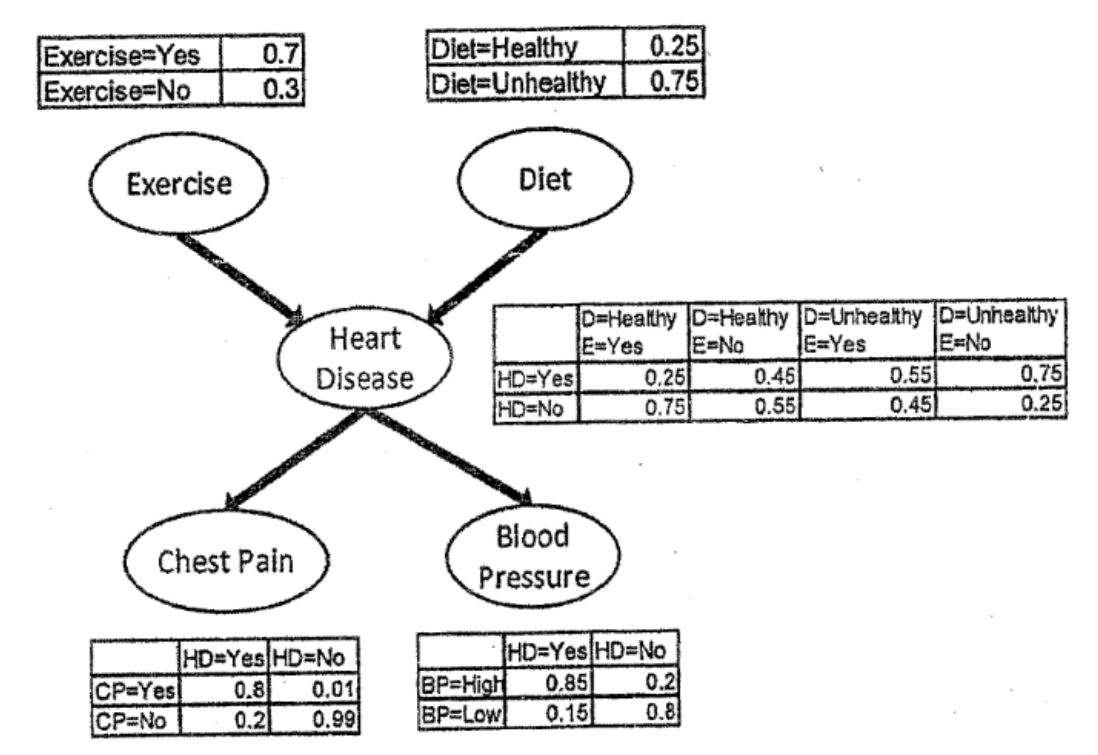
\includegraphics[width=5in]{images/dm_81ba_bbn.png}

      \item Write short notes on: Laplacian Correction in Classification method. \hfill [4] (\bo{78 Bh})
    \end{enumerate}

  \subsection{Artificial Neural Network Classifier}
    \begin{enumerate}[topsep=0pt, noitemsep]
      \item How does Neural Net work classified work? Explain with suitable example. \hfill [8] (81 Ba)
        \lb How ANN works? Explain with Algorithm. \hfill [8] (\bo{75 Ch})
        \lb What is an ANN classifier? Explain its general consideration that required for the classifier. \hfill [2+6] (72 Ka)

      \item Consider the multi-layer feed-forward neural network shown in the following figure. This neural network has three inputs $(x_1)$, $(x_2)$ and $(x_3)$ connected to a hidden layer consisting of two nodes $(h_1)$ and $(h_2)$. The weight of the edge connecting $(x_i)$ to $(h_j)$ is $(w_{ji})$. The two hidden nodes are connected to the output node $(o)$. The weight of the edge connecting the hidden node $(h_i)$ to the output node $(o)$ is $(u_i)$. The activation functions at hidden and output layers is set to sigmoid function defined as follows: \hfill [2+3+4] (\bo{76 Ch})
        \[ \sigma(\theta) = \frac{1}{1 + \exp(-\theta)} \]
        Using the target output $(t)$, the squared error is used as the loss function at the output node, and is defined as:
        \[ E(o,t) = \frac{1}{2}(o-t)^2 \]
        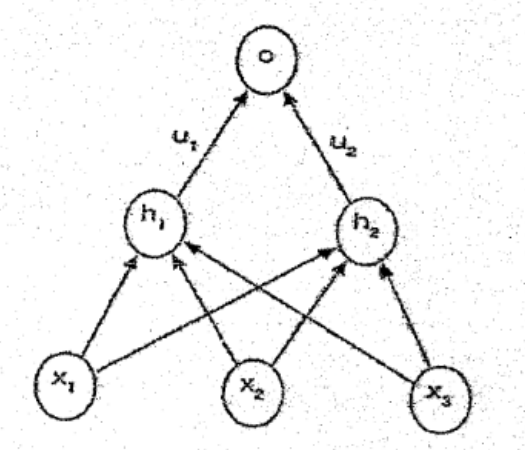
\includegraphics[width=2.6in]{images/dm_76ch_ann.png}
        \begin{enumerate}[label=(\alph*),topsep=2pt,noitemsep]
          \item Using the symbols given above, compute the activation at $(h_1)$.
          \item Compute the gradient of the loss with respect to the output $(o)$.
          \item Compute the gradient of the loss with respect to the weight $(w_{12})$.
        \end{enumerate}

      \item Write short notes on: Neural Network Classifier. \hfill [5] (80 Ba) [5] (\bo{82 Bh})
    \end{enumerate}

  \subsection{Issues: Overfitting, Validation, Model Comparison}
    \begin{enumerate}[topsep=0pt, noitemsep]
      \item Describe the working mechanism as well as the merits and demerits of the holdout method, random sampling, k-cross validation and bootstrap approaches in evaluating the performance of a classifier. \hfill [8] (79 Ba)

      \item Given the following confusion matrix, determine Accuracy, Error rate, Sensitivity, Specificity, Precision, Recall of the classifier model. \hfill [4] (79 Ba)\\
        \small
        \begin{tabular}{|c|c|c|c|}
          \hline
          $n = 165$ & Predicted: NO & Predicted: YES & \\ \hline
          Actual: NO & TN = 50 & FP = 10 & 60 \\ \hline
          Actual: YES & FN = 5 & TP = 100 & 105 \\ \hline
           & 55 & 110 & \\ \hline
        \end{tabular}
        \normalsize

      \item What is ID3 algorithm? Calculate TPR, FPR and Accuracy for given confusion matrix. \hfill [2+6] (\bo{73 Ch})\\
        \small
        \begin{tabular}{|c|c|c|}
          \hline
           & Predicted + & Predicted -- \\ \hline
          Predicted + & 100 & 40 \\ \hline
          Predicted -- & 60 & 300 \\ \hline
        \end{tabular}
        \normalsize\\
        (The paper labels \emph{both} axes ``Predicted''; the row stubs should read ``Actual''. Reproduced as printed.)

      \item In what cases you cannot use Accuracy for performance measure, give some examples. Assume that you have the following confusion matrix. Calculate the Classification error, Sensitivity, False alarm rate Specificity. \hfill [3+5] (80 Ba)\\
        \small
        \begin{tabular}{|c|c|c|c|}
          \hline
          \multicolumn{2}{|c|}{} & \multicolumn{2}{c|}{Actual Values} \\ \cline{3-4}
          \multicolumn{2}{|c|}{} & True & False \\ \hline
          Predicated & True & 1050 & 250 \\ \cline{2-4}
          Values & False & 150 & 950 \\ \hline
        \end{tabular}
        \normalsize

      \item Calculate: Accuracy, TPR, FPR and Precision for the given confusion matrix for a classifier. \hfill [4] (\bo{78 Bh})\\
        \small
        \begin{tabular}{|c|c|c|c|}
          \hline
          \multicolumn{2}{|c|}{} & \multicolumn{2}{c|}{Actual Class} \\ \cline{3-4}
          \multicolumn{2}{|c|}{} & Class 1 & Class 2 \\ \hline
          Predicted & Class 1 & 142 & 40 \\ \cline{2-4}
          Class & Class 2 & 98 & 720 \\ \hline
        \end{tabular}
        \normalsize

      \item The confusion matrix for a classifier is given as follows. Calculate: Accuracy, Sensitivity, Specificity and Precision. \hfill [10] (75 Ash)\\
        \small
        \begin{tabular}{|c|c|c|c|}
          \hline
          \multicolumn{2}{|c|}{} & \multicolumn{2}{c|}{Predicted Class} \\ \cline{3-4}
          \multicolumn{2}{|c|}{} & Class 1 & Class 2 \\ \hline
          Actual & Class 1 & 21 & 6 \\ \cline{2-4}
          Class & Class 2 & 7 & 41 \\ \hline
        \end{tabular}
        \normalsize

      \item The confusion matrix for a classifier is given as follows. Calculate: a) Accuracy \quad b) Sensitivity \quad c) Specificity \quad d) Precision \hfill [10] (74 Ash)\\
        \small
        \begin{tabular}{|c|c|c|c|}
          \hline
          \multicolumn{2}{|c|}{} & \multicolumn{2}{c|}{Predicted Class} \\ \cline{3-4}
          \multicolumn{2}{|c|}{} & Class 1 & Class 2 \\ \hline
          Actual & Class 1 & 25 & 9 \\ \cline{2-4}
          Class & Class 2 & 4 & 31 \\ \hline
        \end{tabular}
        \normalsize

      \item The confusion matrix for a classifier is given as follows. Calculate a. accuracy \quad b. sensitivity \quad c. specificity \quad d. precision \quad e. recall \hfill [10] (\bo{72 Ch})\\
        \small
        \begin{tabular}{|c|c|c|c|}
          \hline
          \multicolumn{2}{|c|}{} & \multicolumn{2}{c|}{actual class} \\ \cline{3-4}
          \multicolumn{2}{|c|}{} & class1 & class2 \\ \hline
          predicted & class1 & 21 & 6 \\ \cline{2-4}
          class & class2 & 7 & 41 \\ \hline
        \end{tabular}
        \normalsize

      \item Explain ROC. Using the following data, calculate TPR, FPR, precision for given confusion matrix. Classify, A = Yes, B = No. \hfill [1+3+6] (73 Shr)\\
        \small
        \begin{tabular}{|c|c|c|}
          \hline
           & A & B \\ \hline
          A & 20 & 5 \\ \hline
          B & 10 & 40 \\ \hline
        \end{tabular}
        \normalsize

      \item An input sequence ``A A B B B A A A B B'' was used for classification. The Classifier `X' predicted the sequences as: ``A A B B B A A A B B'' where as the Classifier `Y' predicted the sequences as: ``A A A A B B A A A B''. Develop the corresponding confusion matrix for the classifiers and find their corresponding. \hfill [10] (\bo{70 Ch})
        \begin{enumerate}[label=\roman*),topsep=2pt,noitemsep]
          \item Accuracy
          \item Precision
          \item True Positive Rate
          \item False Positive Rate
        \end{enumerate}

      \item Write short notes on: Overfitting problem in classification. \hfill [4] (\bo{78 Bh})
        \lb Write short notes on: Overfitting and ROC. \hfill [4] (\bo{73 Ch})
    \end{enumerate}

\pagebreak
%=======================================================================
\section{Association Analysis}
\begin{center}(10 Hours)\end{center}

  \subsection{Basics and Algorithms}
    \begin{enumerate}[topsep=0pt, noitemsep]
      \item What is an association analysis? Explain its importance in market-basket analysis. \hfill [2+5] (72 Ka)
        \lb What is the use of Apriori Algorithm in market basket analysis? Explain with suitable example. \hfill [10] (\bo{72 Ch})
        \lb Where is association analysis applicable and beneficial for us? Elaborate FP Growth Method Algorithm with examples. \hfill [2+6] (80 Ba)
        \lb What are association rules? Explain its importance with example. \hfill [6] (70 Asa)

      \item Why association analysis is required in data mining? Explain Apriori principle with example. \hfill [2+6] (75 Ash) [2+6] (\bo{74 Ch})

      \item What is the importance of SUPPORT and COFIDENCE during association analysis? Explain FP-Growth method with example. \hfill [10] (\bo{72 Ch})
        \lb Explain the term support and confidence in association analysis. (asked with the Apriori numerical --- full statement in 4.2) \hfill [2] (\bo{82 Bh})

      \item Why is pattern evaluation important in association rule mining? Explain with example the statistical based measures used for measuring interestingness of association rules. \hfill [8] (\bo{70 Ch})

      \item Generally, we will be more interested in associated rules with high confidence. However, often we will not be interested in association rules that have a confidence of 100\%. Why? Then specifically explain why association rules with 99\% confidence may be interesting (i.e., what might they indicate)? \hfill [4] (80 Ba) --- asked with the Apriori numerical, full statement in 4.2

      \item Write short notes on: Market Basket Analysis. \hfill [4] (\bo{75 Ch})
    \end{enumerate}

  \subsection{Frequent Itemset Pattern \& Apriori Principle}
    \begin{enumerate}[topsep=0pt, noitemsep]
      \item What is Association Analysis? Explain with different use cases? Use the Apriori algorithm to find the frequent itemsets. Assume minimum support count is 4 and confidence is 80\%. \hfill [2+7] (\bo{80 Bh})\\
        \small
        \begin{tabular}{|c|l|}
          \hline
          TID & Items \\ \hline
          T100 & F, A, C, D, G, I, M, P, N \\ \hline
          T101 & A, B, C, D, F, L, M, O, P \\ \hline
          T102 & B, F, H, V, J, O, P \\ \hline
          T103 & B, C, K, S, A, V \\ \hline
          T104 & L, A, F, C, E, P, M, N, V \\ \hline
          T105 & I, B, A, P, S, M \\ \hline
          T106 & F, A, C, I, B, A, P \\ \hline
        \end{tabular}
        \normalsize

      \item Explain the term support and confidence in association analysis. Derive association rule for following transaction considering minimum support = 60\% and confidence = 80\% using Apriori Algorithm. \hfill [2+8] (\bo{82 Bh})\\
        \small
        \begin{tabular}{|c|l|}
          \hline
          TID & Transaction \\ \hline
          T1 & A, B, C, D, E, F \\ \hline
          T2 & B, C, D, E, F, G \\ \hline
          T3 & A, D, E, H \\ \hline
          T4 & A, D, F, I, J \\ \hline
          T5 & B, D, E, K \\ \hline
        \end{tabular}
        \normalsize

      \item For the transaction given below, consider Confidence = 65\% and minimum support = 50\%. Identify frequent itemsets with possible association rules using Apriori Algorithm. \hfill [2+6] (\bo{81 Bh})\\
        \small
        \begin{tabular}{|c|l|}
          \hline
          TID & Items \\ \hline
          1 & MILK, BREAD, CAKE \\ \hline
          2 & BUTTER, BREAD, EGG \\ \hline
          3 & MILK, BUTTER, BREAD, EGG \\ \hline
          4 & BUTTER, EGG \\ \hline
        \end{tabular}
        \normalsize

      \item (a) Write Apriori algorithm and using the algorithm find all the frequent itemset for the following database. (min\_sup = 20\%). \hfill [5+3] (79 Ba)\\
        \small
        \begin{tabular}{|c|c|c|c|c|c|c|c|c|c|}
          \hline
          TID & A1 & A2 & A3 & A4 & A5 & A6 & A7 & A8 & A9 \\ \hline
          T2 & 0 & 1 & 0 & 1 & 0 & 0 & 0 & 1 & 0 \\ \hline
          T3 & 0 & 0 & 0 & 1 & 1 & 0 & 1 & 0 & 0 \\ \hline
          T4 & 0 & 0 & 1 & 0 & 0 & 0 & 0 & 0 & 0 \\ \hline
          T5 & 0 & 0 & 0 & 0 & 1 & 1 & 1 & 0 & 0 \\ \hline
          T6 & 0 & 1 & 1 & 1 & 0 & 0 & 0 & 0 & 0 \\ \hline
          T7 & 0 & 1 & 0 & 0 & 0 & 1 & 1 & 0 & 1 \\ \hline
          T8 & 0 & 0 & 0 & 0 & 1 & 0 & 0 & 0 & 0 \\ \hline
        \end{tabular}
        \normalsize\\
        (The table as printed starts at T2 --- there is no T1 row --- and heads its eighth column ``AB'', a broken ``A8''.)
        \begin{itemize}[topsep=2pt,noitemsep,label={}]
          \item (b) Is it possible to generate any rules out of the frequent items, considering any value of confidence threshold?
        \end{itemize}

      \item Explain Apriori algorithm in market basket analysis? Derive association rule from the following market basket transactions with 50\% of minimum support and confidence respectively. \hfill [3+7] (\bo{73 Ch})\\
        \small
        \begin{tabular}{|c|l|}
          \hline
          Transaction & Itemsets \\ \hline
          1 & A, B, C \\ \hline
          2 & A, C \\ \hline
          3 & A, D \\ \hline
          4 & B, E, F \\ \hline
        \end{tabular}
        \normalsize

      \item Generally, we will be more interested in associated rules with high confidence. However, often we will not be interested in association rules that have a confidence of 100\%. Why? Then specifically explain why association rules with 99\% confidence may be interesting (i.e., what might they indicate)? Identify the candidate and large item sets of the following transaction table using Apriori algorithm with minimum support 2. \hfill [4+5] (80 Ba)\\
        \small
        \begin{tabular}{|c|l|}
          \hline
          TID & Items \\ \hline
          10 & A, C, D \\ \hline
          20 & B, C, E \\ \hline
          30 & A, B, C, E \\ \hline
          40 & B, E \\ \hline
        \end{tabular}
        \normalsize

      \item Derive association rule for the following market basket transactions. Minimum support = 50\%, Minimum confidence = 80\%. \hfill [8] (\bo{79 Bh})\\
        \small
        \begin{tabular}{|c|l|}
          \hline
          Transaction ID & Item Set \\ \hline
          1 & A,B \\ \hline
          2 & A,D \\ \hline
          3 & A,C \\ \hline
          4 & B,E \\ \hline
          5 & B,D,E \\ \hline
          6 & A,E,C \\ \hline
        \end{tabular}
        \normalsize

      \item Consider the transaction data shown in the following table from a fast food restaurant. \hfill [5+3] (\bo{76 Ch})\\
        \small
        \begin{tabular}{|c|l|}
          \hline
          Meal Item & List of Item IDs \\ \hline
          Order:1 & M1, M2, M5 \\ \hline
          Order:2 & M2, M4 \\ \hline
          Order:3 & M2, M3 \\ \hline
          Order:4 & M1, M2, M4 \\ \hline
          Order:5 & M1, M3 \\ \hline
          Order:6 & M2, M3 \\ \hline
          Order:7 & M1, M3 \\ \hline
          Order:8 & M1, M2, M3, M5 \\ \hline
          Order:9 & M1, M2, M3 \\ \hline
        \end{tabular}
        \normalsize\\
        There are 9 distinct transactions (Order: 1 -- Order: 9) and each transaction involves between 2 and 4 meal items. There are a total of 5 meal items that are involved in the transactions. For simplicity, the meal items have been assigned short names (M1-M5). Assume that the minimum support is 2/9 and the minimum confidence is 7/9.
        \begin{enumerate}[label=(\alph*),topsep=2pt,noitemsep]
          \item Apply the Apriori algorithm to the dataset of transactions and identify all frequent k-itemsets.
          \item Find all strong association rules of the form: $X \wedge Y \rightarrow Z$ and note their confidence values.
        \end{enumerate}

      \item For the transactions given below, consider confidence=60\% and minimum support=30\%. Identify large itemsets (L-Itemset) at L=3 with possible associations using A-priori algorithm and generate F-List using FP-Growth algorithm. \hfill [12] (76 Ash)\\
        \small
        \begin{tabular}{|c|l|}
          \hline
          Transactions & Items description \\ \hline
          T1 & A, B, C, T, M, P, D, K \\ \hline
          T2 & A, B, T, P, D, K \\ \hline
          T3 & B, C, T, D, M, A, P \\ \hline
          T4 & A, C, T, M, D, \\ \hline
          T5 & A,C, D, K, M \\ \hline
          T6 & B, C, T \\ \hline
        \end{tabular}
        \normalsize

      \item Identify the candidate, frequent item sets and association rules for the following transaction data using Apriori algorithm. Take minimum support = 20\%, minimum confidence 80\%. \hfill [8] (74 Ash)\\
        \small
        \begin{tabular}{|c|l|}
          \hline
          TID & ITEMS \\ \hline
          1 & M1, M2, M5 \\ \hline
          2 & M2, M4 \\ \hline
          3 & M2, M3 \\ \hline
          4 & M1, M2, M4 \\ \hline
          5 & M1, M3 \\ \hline
          6 & M2, M3 \\ \hline
          7 & M1, M3 \\ \hline
          8 & M1, M2, M3, M5 \\ \hline
          9 & M1, M2, M3 \\ \hline
        \end{tabular}
        \normalsize

      \item Explain Apriori algorithm. Use Apriori to generate frequent item sets with support of 50\% for the following transaction database. \hfill [10] (\bo{70 Ch})\\
        \small
        \begin{tabular}{|c|l|}
          \hline
          TID & Items \\ \hline
          1 & ACD \\ \hline
          2 & BD \\ \hline
          3 & ABCE \\ \hline
          4 & BDF \\ \hline
        \end{tabular}
        \normalsize

      \item How does Apriori Algorithm optimize the brute force approach for frequent item set generation? \hfill [10] (\bo{71 Ch})
        \lb What is frequent item set mining? How do Apriori and FP-growth algorithm optimize the brute force approach for finding frequent item sets? \hfill [15] (\bo{69 Ch})

      \item What are association rules? How can spriori algorithm be used to generate association rules. \hfill [10] (71 Shr)
        \lb How can Apriori Algorithm be used for finding association rules out of a frequent item set? \hfill [7] (\bo{69 Ch})
    \end{enumerate}

  \subsection{FP-Growth, FP-Tree}
    \begin{enumerate}[topsep=0pt, noitemsep]
      \item What is FP-Growth Algorithm? Explain FP-Growth Algorithm with example. \hfill [2+5] (\bo{80 Bh})
        \lb Explain FP-Growth algorithm with example. \hfill [8] (74 Ash)
        \lb Explain FP-growth algorithm in detail. \hfill [10] (71 Shr)
        \lb What are the advantages of FP growth method? Explain FP growth algorithm. \hfill [2+6] (75 Ash)
        \lb What is a Frequent item set? Explain FP growth method with example. \hfill [1+8] (72 Ka)
        \lb When do we use Association analysis? Explain FP-Tree with an example. \hfill [2+5] (81 Ba)
        \lb What are the advantages of FP-Growth Algorithm over Apriori Algorithm? Explain FP-Growth Algorithm for finding frequent patterns with suitable example. \hfill [2+6] (\bo{81 Bh})
        \lb How does FP growth approach generate frequent item sets without generating candidate item sets? Explain with an example. \hfill [6] (79 Ba)
        \lb What is the use of FP-Growth method in market basket analysis? Explain FP-Growth method with a suitable example. \hfill [10] (\bo{73 Ch})
        \lb Explain FP growth algorithm in detail with example. \hfill [12] (70 Asa)
        \lb What do you mean by frequent Pattern growth, draw FP-tree with given tabular data. \hfill [4+4] (\bo{75 Ch})\\
        \small
        \begin{tabular}{|c|l|}
          \hline
          TID & Items \\ \hline
          01 & f, a, c, d, g, i, m, p \\ \hline
          02 & a, b, c, f, l, m, o \\ \hline
          03 & b, f, h, j, o, w \\ \hline
          04 & b, c, k, s, p \\ \hline
          05 & A, f, c, e, l, p, m, n \\ \hline
        \end{tabular}
        \normalsize

      \item What is limitation of Apriori algorithm compared to FP-growth? A database has 5 transactions, given in table below. Let min support = 60\% and min confidence = 80\%. \hfill [2+7] (81 Ba)\\
        \small
        \begin{tabular}{|c|l|}
          \hline
          TID & Item\_bought \\ \hline
          T100 & \{M, O, N, K, E, Y\} \\ \hline
          T200 & \{D, O, N, K, E, Y\} \\ \hline
          T300 & \{M, A, K, E\} \\ \hline
          T400 & \{M, U, C, K, Y\} \\ \hline
          T500 & \{C, O, O, K, I, E\} \\ \hline
        \end{tabular}
        \normalsize
        \begin{enumerate}[label=\roman*),topsep=2pt,noitemsep]
          \item Find all frequent itemsets using FP-growth.
          \item List all of the strong association rules (with support and confidence).
        \end{enumerate}

      \item Consider the given transactional database from a grocery store. Use a support threshold of 33.34\% and confidence threshold of 60\% to compute the following: \hfill [4+4] (\bo{78 Bh})\\
        \small
        \begin{tabular}{|c|l|}
          \hline
          Transcation ID & Items \\ \hline
          T1 & HotDogs, Buns, Ketchup \\ \hline
          T2 & HotDogs, Buns \\ \hline
          T3 & HotDogs, Coke, Chips \\ \hline
          T4 & Chips, Coke \\ \hline
          T5 & Chips, Ketchup \\ \hline
          T6 & HotDogs, Coke, Chips \\ \hline
        \end{tabular}
        \normalsize
        \begin{enumerate}[label=\alph*),topsep=2pt,noitemsep]
          \item Build a frequent pattern tree (FP-Tree). Show for each transaction how the tree evolves.
          \item Use FP-Growth algorithm to discover the frequent itemsets from this FP-tree.
        \end{enumerate}

      \item How does FP growth approach overcomes the disadvantages of Apriori algorithm. For the transaction data given in table generate FP-Tree. \hfill [2+8] (\bo{74 Ch})\\
        \small
        \begin{tabular}{|c|l|}
          \hline
          Transaction ID & Item set \\ \hline
          T1 & Camera, Laptop, Pen drive \\ \hline
          T2 & Laptop, Pen drive \\ \hline
          T3 & Laptop, Mobile, Earphone \\ \hline
          T4 & Earphone, Mobile \\ \hline
          T5 & Camera, Earphone \\ \hline
          T6 & Laptop, Mobile, Earphone \\ \hline
        \end{tabular}
        \normalsize

      \item What is FP Tree? How FP-growth algorithm eliminate the problem of Apriori algorithm? Construct the FP tree and find association rules for the following transaction database using FG- Growth algorithm. Support = 30\% and confidence = 75\%. \hfill [10] (73 Shr)\\
        \small
        \begin{tabular}{|c|l|}
          \hline
          Transaction ID & Items \\ \hline
          1 & P,R,S \\ \hline
          2 & R,S,T \\ \hline
          3 & P,Q,R \\ \hline
          4 & P,R,S,T \\ \hline
          5 & P,S,T \\ \hline
          6 & P,Q,T \\ \hline
          7 & Q,S,T \\ \hline
          8 & Q,R,T \\ \hline
        \end{tabular}
        \normalsize

      \item Write short notes on: FP-Tree. \hfill [5] (\bo{79 Bh})
        \lb Write short notes on: FP Growth Algorithm. \hfill [5] (\bo{82 Bh})
    \end{enumerate}

  \subsection{Handling Categorical Attributes}
    \begin{enumerate}[topsep=0pt, noitemsep]
      \item How do you handle the categorical attributes in data mining process? Explain with example. Generate the at least four subsequences from the given sequence: $<$ \{2,3,5\}, \{6,7,8\}, \{9,1\}, \{7,4\} $>$. \hfill [3+3] (\bo{79 Bh})

      \item What are Categorical data? What are the possible issues arrives when using Categorical data? How can you handle such issues? \hfill [2+3+3] (73 Shr)

      \item Write short notes on: Categorical data and related issues. \hfill [4] (\bo{72 Ch})
    \end{enumerate}

  \subsection{Sequential, Subgraph, and Infrequent Patterns}
    \begin{enumerate}[topsep=0pt, noitemsep]
      \item (a) List all the 4-subsequences contained in the data sequence: $<$ \{1,3\} \{2\} \{2,3\} \{4\} $>$ \hfill [3+3] (\bo{76 Ch})\\
        (b) Draw all candidate sub-graphs obtained from joining the pair of graphs shown below using edge-growing method to expand the sub-graphs.\\
        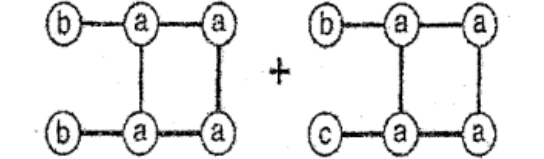
\includegraphics[width=3.6in]{images/dm_76ch_subgraph.png}

      \item What are subgraph pattern? \hfill [2] (\bo{79 Bh})

      \item Explain Sequential Pattern and Sub-graph Pattern with suitable example. \hfill [4+4] (\bo{73 Ch})

      \item Write short notes on: AprioriALL: Sequential pattern mining algorithm. \hfill [3] (76 Ash)

      \item Write short notes on: Sequential pattern. \hfill [3] (72 Ka)
    \end{enumerate}

\pagebreak
%=======================================================================
\section{Cluster Analysis}
\begin{center}(9 Hours)\end{center}

  \subsection{Basics and Algorithms}
    \begin{enumerate}[topsep=0pt, noitemsep]
      \item What is Cluster Analysis? What are its applications? Explain different types of clusters. \hfill [8] (81 Ba)
        \lb What is a cluster analysis? How it is different from classification? \hfill [5] (72 Ka)
        \lb What is the application of clustering in data mining? Explain K-means clustering with example. \hfill [2+6] (\bo{75 Ch})
        \lb What is the application of clustering in data mining? Explain the k-means algorithm with example. \hfill [8] (73 Shr)
        \lb When do we use clustering? How do you evaluate the cluster generated? \hfill [3+4] (\bo{80 Bh})
        \lb How clustering differ from classification? (asked with the 1-D K-means / SSE numerical --- full statement in 5.2) \hfill [4] (\bo{73 Ch})

      \item Why is a clustering an unsupervised learning? How can hierarchical clusters be generated using Bisecting K-means algorithm? \hfill [10] (\bo{71 Ch})

      \item What are the types of clustering methods? Explain DBSCAN method of clustering with an example. \hfill [10] (\bo{72 Ch})
        \lb List the various types of partition based clustering methods. Explain Hierarchical clustering method with an example. \hfill [10] (74 Ash)

      \item What is contiguous cluster? Explain an algorithm that can be used to generate contiguous clusters. \hfill [10] (71 Shr)

      \item An internet marketer is interesting in segmenting internet based the input attributes --- top ten search key words used, top 10 URLs, recent 10 online purchases (vendor, product, qty, amt), Internet usage level, heaviest access hour, and heaviest access day of a week. Which clustering algorithm do you think can be used for segmentation? How do you validate the cluster which has been created? \hfill [2+6] (\bo{79 Bh})
    \end{enumerate}

  \subsection{K-means Clustering}
    \begin{enumerate}[topsep=0pt, noitemsep]
      \item Describe K-means algorithm for clustering and discuss strategy in determining the optimal value of K. \hfill [4+4] (80 Ba)
        \lb Explain K-means clustering algorithm with examples. \hfill [10] (\bo{69 Ch})

      \item Use K-means clustering to cluster the following given data for K = 2 with Euclidean distance matrix. List down the demerits of this algorithm. \hfill [5+3] (81 Ba)\\
        (The paper prints no data table for this question.)

      \item Describe the K-means clustering algorithm. Generate two clusters from following dataset using K-means clustering. \hfill [2+8] (\bo{82 Bh})\\
        \small
        \begin{tabular}{|c|c|c|}
          \hline
          Instance & A & B \\ \hline
          1 & 1 & 2 \\ \hline
          2 & 1.5 & 1 \\ \hline
          3 & 3.5 & 1.5 \\ \hline
          4 & 4 & 3 \\ \hline
          5 & 3.5 & 2.5 \\ \hline
          6 & 6 & 4 \\ \hline
        \end{tabular}
        \normalsize

      \item Consider the data points $\{(2,3), (3,3), (6,8), (8,8), (7,5)\}$ with initial centroid (2,3). Apply K-means algorithm to choose the next centroid and cluster these data points into k = 2. Discuss the problems that arise with K-means clustering algorithm and ways to solve it. \hfill [5+3] (\bo{81 Bh})

      \item Define clustering. Given the matrix whose column represent different data points, perform a K-means clustering on this dataset using the Manhattan as the distance function. The center of the 3 clusters are initiated as A(6.2, 3.2), B(6.6, 3.7) and C(6.5, 3.0). Provide the final cluster centers after 3 iteration. \hfill [8] (79 Ba)
        \[ \begin{bmatrix}
          5.9 & 4.6 & 6.2 & 4.7 & 5.5 & 5.0 & 4.9 & 6.7 & 5.1 & 6.0 \\
          3.2 & 2.9 & 2.8 & 3.2 & 4.2 & 3.0 & 3.1 & 3.1 & 3.8 & 3.0
        \end{bmatrix} \]

      \item How clustering differ from classification? Given the one-dimensional points $\{5, 12, 18, 24, 30, 42, 48\}$ with initial centroids $\{5, 12, 18\}$, create three clusters by K-Means algorithm and calculate SSE for this clustering result. \hfill [4+8] (\bo{73 Ch})

      \item Write K-means clustering algorithm. Generate two clusters from following dataset using K-means clustering. \hfill [2+6] (\bo{78 Bh})\\
        \small
        \begin{tabular}{|c|c|c|}
          \hline
          Instance & A & B \\ \hline
          1 & 1 & 2 \\ \hline
          2 & 2.5 & 1 \\ \hline
          3 & 3.5 & 1.5 \\ \hline
          4 & 4 & 1 \\ \hline
          5 & 3.5 & 2.5 \\ \hline
          6 & 5 & 3 \\ \hline
        \end{tabular}
        \normalsize

      \item Write K-means algorithm and find clusters for following data set. (Take K = 2) \hfill [2+8] (74 Ash)\\
        \small
        \begin{tabular}{|c|c|c|}
          \hline
          Instance & X & Y \\ \hline
          1 & 1.0 & 2.0 \\ \hline
          2 & 2.5 & 1.0 \\ \hline
          3 & 3.5 & 1.5 \\ \hline
          4 & 4.0 & 1.0 \\ \hline
          5 & 3.5 & 2.5 \\ \hline
          6 & 5.0 & 3.0 \\ \hline
        \end{tabular}
        \normalsize

      \item Explain K-means clustering with limitation. Generate two clusters from following dataset using K-means clustering. \hfill [4+6] (75 Ash)\\
        \small
        \begin{tabular}{|c|c|}
          \hline
          A & B \\ \hline
          1 & 2 \\ \hline
          2.5 & 4.5 \\ \hline
          4 & 6 \\ \hline
          3.5 & 4 \\ \hline
          4 & 5.5 \\ \hline
          3 & 6 \\ \hline
        \end{tabular}
        \normalsize

      \item Explain K-means clustering with limitation Use k-means clustering to cluster the following dataset. \hfill [10] (71 Shr)\\
        \small
        \begin{tabular}{|c|c|}
          \hline
          A & B \\ \hline
          1.0 & 1.0 \\ \hline
          1.5 & 2.0 \\ \hline
          3.0 & 4.0 \\ \hline
          5.0 & 7.0 \\ \hline
          3.5 & 5.0 \\ \hline
          4.5 & 5.0 \\ \hline
          3.5 & 4.5 \\ \hline
        \end{tabular}
        \normalsize

      \item Given the matrix $(X)$ whose rows represent different data points, perform a k-means clustering on this dataset using the Euclidean distance as the distance function. Here $(K)$ is chosen as 3. The center of the 3 clusters are initialized as red (6.2, 3.2), green (6.6, 3.7) and blue (6.5, 3.0). Provide the final cluster centers and comment on the number of iterations required for the clusters to converge. \hfill [8] (\bo{76 Ch})
        \[ X = \begin{bmatrix}
          5.9 & 3.2 \\ 4.6 & 2.9 \\ 6.2 & 2.8 \\ 4.7 & 3.2 \\ 5.5 & 4.2 \\
          5.0 & 3.0 \\ 4.9 & 3.1 \\ 6.7 & 3.1 \\ 5.1 & 3.8 \\ 6.0 & 3.0
        \end{bmatrix} \]

      \item Describe the difference between Hierarchical and partitioning clustering. How K-means clustering is applied? Verify using example. \hfill [2+8] (\bo{74 Ch})
    \end{enumerate}

  \subsection{Hierarchical Clustering}
    \begin{enumerate}[topsep=0pt, noitemsep]
      \item What is hierarchical clustering? Use this clustering approach to draw dendrogram for given data points. \hfill [2+7] (\bo{80 Bh})\\
        \small
        \begin{tabular}{|c|c|c|c|c|c|c|}
          \hline
           & p1 & p2 & p3 & p4 & p5 & p6 \\ \hline
          p1 & 0.00 & 0.24 & 0.22 & 0.37 & 0.34 & 0.23 \\ \hline
          p2 & 0.24 & 0.00 & 0.15 & 0.20 & 0.14 & 0.25 \\ \hline
          p3 & 0.22 & 0.15 & 0.00 & 0.15 & 0.28 & 0.11 \\ \hline
          p4 & 0.37 & 0.20 & 0.15 & 0.00 & 0.29 & 0.22 \\ \hline
          p5 & 0.34 & 0.14 & 0.28 & 0.29 & 0.00 & 0.39 \\ \hline
          p6 & 0.23 & 0.25 & 0.11 & 0.22 & 0.39 & 0.00 \\ \hline
        \end{tabular}
        \normalsize

      \item Cluster the following samples based on complete-linkage algorithm and draw the dendrogram. Using Euclidean distance. \hfill [8] (80 Ba)\\
        \small
        \begin{tabular}{|c|c|c|}
          \hline
          Point & x Coordinate & y Coordinate \\ \hline
          p1 & 0.40 & 0.53 \\ \hline
          p2 & 0.22 & 0.38 \\ \hline
          p3 & 0.35 & 0.32 \\ \hline
          p4 & 0.26 & 0.19 \\ \hline
          p5 & 0.08 & 0.41 \\ \hline
          p6 & 0.45 & 0.30 \\ \hline
        \end{tabular}
        \normalsize

      \item The table below is a distance matrix for six objects: \hfill [4+4] (\bo{76 Ch})\\
        \small
        \begin{tabular}{|c|c|c|c|c|c|c|}
          \hline
           & A & B & C & D & E & F \\ \hline
          A & 0 & & & & & \\ \hline
          B & 0.12 & 0 & & & & \\ \hline
          C & 0.51 & 0.25 & 0 & & & \\ \hline
          D & 0.84 & 0.16 & 0.14 & 0 & & \\ \hline
          E & 0.28 & 0.77 & 0.70 & 0.45 & 0 & \\ \hline
          F & 0.34 & 0.61 & 0.93 & 0.20 & 0.67 & 0 \\ \hline
        \end{tabular}
        \normalsize
        \begin{enumerate}[label=(\alph*),topsep=2pt,noitemsep]
          \item Show the final result of hierarchical clustering with single-link by drawing a dendrogram.
          \item Show the final result of hierarchical clustering with complete-link by drawing a dendrogram.
        \end{enumerate}

      \item What is Hierarchical Clustering? Differentiate between agglomerative and divisive approach of hierarchical clustering. Augment your answer with appropriate illustrative examples. \hfill [10] (\bo{70 Ch})

      \item Explain hierarchical clustering method with an example of Dendogram plot. \hfill [6] (79 Ba)
    \end{enumerate}

  \subsection{DBSCAN Clustering}
    \begin{enumerate}[topsep=0pt, noitemsep]
      \item What are core, border and noise points? Write the algorithm of DBSCAN clustering and explain how it is useful in handling the noisy data. \hfill [3+5] (\bo{79 Bh})
        \lb How DBSCAN clustering is used for handling noise in data? \hfill [8] (\bo{75 Ch})
        \lb How DBSCAN algorithm works? How do we avoid the issues of DBSCAN? \hfill [8+2] (76 Ash)
        \lb Explain a DBSCAN algorithm with example. \hfill [7] (72 Ka)

      \item What are core, border and noise points? Consider the following points (2, 10), (2, 5), (8, 4), (5, 8), (7, 5), (6, 4), (1, 2), (4, 9). Use DBSCAN algorithm to find cluster with e = 2 and minPts = 2. \hfill [3+5] (\bo{82 Bh})

      \item Provide answers to the following with regard to the DBSCAN clustering approach: \hfill [2+2+2] (\bo{78 Bh})
        \begin{enumerate}[label=\alph*),topsep=2pt,noitemsep]
          \item How does the DBSCAN quantify the neighborhood of an object? How is a large dense region assembled from small dense regions centered by core objects?
          \item How does DBSCAN find clusters? How are the neighborhood threshold (Epsilion) and minimum number of points (MinPts) determined empirically in DBSCAN?
          \item Prove that in DBSCAN, for a fixed minimum number of points (MinPts) value and two neighborhood thresholds, Epsilion1 $<$ Epsilion2, a cluster (C) with respect to Epsilion1 and MinPts must be a subset of a subset of a cluster (K) with respect to Epsilion2 and MinPts.
        \end{enumerate}

      \item What is a density based cluster. Explain an algorithm that can be used to generate density based clusters. \hfill [8] (\bo{70 Ch})
        \lb What are outliers? Explain an algorithm that can be used to generate density based clusters. \hfill [8] (75 Ash)
        \lb What are density based clusters? Explain DBSCAN clustering algorithm with example. \hfill [10] (70 Asa)

      \item Write short notes on: Density reachable and Density Connected. \hfill [4] (74 Ash)

      \item Write short notes on: DBSCAN Clustering. \hfill [4] (\bo{81 Bh}) [4] (79 Ba)
    \end{enumerate}

  \subsection{Issues: Evaluation, Scalability, Comparison}
    \begin{enumerate}[topsep=0pt, noitemsep]
      \item Explain the different measures of cluster validity. \hfill [10] (\bo{71 Ch})
        \lb Explain different measures that can be used to compare two clusters. \hfill [6] (70 Asa)
        \lb Explain the issues regarding cluster validation. \hfill [6] (\bo{69 Ch})

      \item How do you evaluate the cluster generated? (asked with ``When do we use clustering?'' --- see 5.1) \hfill [4] (\bo{80 Bh})

      \item Write short notes on: Issues in clustering. \hfill [3] (\bo{74 Ch})

      \item Write short notes on: Cluster evaluation. \hfill [3] (72 Ka)
    \end{enumerate}

\pagebreak
%=======================================================================
\section{Anomaly / Fraud Detection}
\begin{center}(3 Hours)\end{center}

    \begin{enumerate}[topsep=0pt, noitemsep]
      \item What is anomaly detection? Explain distance based method for anomaly detection. \hfill [2+3] (80 Ba)
        \lb What is anamoly detection? Explain distance based method for anamoly detection. \hfill [8] (73 Shr)
        \lb Why anamoly detection is important? Explain distance based method for anamoly detection. \hfill [2+6] (75 Ash)
        \lb What do you mean by anomaly detection and why is it important? Describe distance based approaches for anomaly detection. \hfill [4+3] (\bo{74 Ch})
        \lb What is an Anomaly Detection? Explain few distance based approaches that can be used for Anomaly Detection. \hfill [10] (\bo{71 Ch})
        \lb What is outlier? Explain the distance base approaches for the anomaly detection. \hfill [5] (\bo{75 Ch})
        \lb What is anomaly detection? Explain distance-based method for anomaly detection. \hfill [2+5] (\bo{82 Bh})

      \item What is Anomaly Detection? Why is Anomaly Detection important? Briefly explain different types of anomaly detection schemes. \hfill [2+2+4] (81 Ba)
        \lb What do you mean by anomaly detection? Why is it important and where is it applicable? \hfill [3+3] (\bo{79 Bh})
        \lb What is an Anomaly detection? Discuss its importance in security. \hfill [5] (72 Ka)
        \lb What do you mean by Anomaly Detection? Explain different approaches for Anomaly Detection. \hfill [2+6] (\bo{81 Bh})

      \item What is anomaly desertion? Explain likelihood approach for anomaly detection. \hfill [8] (70 Asa)

      \item Explain different types of outlier with suitable examples. How density based outlier detection works? \hfill [5+3] (\bo{80 Bh})

      \item Compare and contrast among three difference methods of anomaly detection. \hfill [6] (\bo{78 Bh})
        \lb Describe the strengths and weaknesses of the statistical, proximity-based, density-based and cluster-based approaches of anomaly detection. \hfill [6] (79 Ba)

      \item (a) Discuss the issues related to anomaly detection. \hfill [2] (\bo{76 Ch})\\
        (b) If the probability that a normal object is classified as an anomaly is 0.01 and the probability that an anomalous object is classified as anomalous is 0.99, then what is the false alarm rate and detection rate if 99\% of the objects are normal? \hfill [3] (\bo{76 Ch})
        \lb What is anomaly detection? Explain the issues associated with anomaly detection. \hfill [2+3] (\bo{73 Ch})

      \item How can Nearest-Neighbor algorithm be used for anomaly defection? \hfill [10] (71 Shr)

      \item What is Base Rate Fallacy? Explain with example. \hfill [7] (\bo{69 Ch})

      \item Write short notes on: Clustering and its application in anomaly detection. \hfill [3] (76 Ash)

      \item Write short notes on: Issues in anomaly/Fraud detection. \hfill [4] (\bo{72 Ch})

      \item Write short notes on: Data Mining for Anomy Detection. \hfill [4] (74 Ash)

      \item Write short notes on: Anomaly Detection; Base Rate Fallacy; Convex Hull Method. \hfill [15] (\bo{70 Ch})
    \end{enumerate}

\pagebreak
%=======================================================================
\section{Advanced Applications}
\begin{center}(3 Hours)\end{center}

  \subsection{Mining Object and Multimedia}
    \begin{enumerate}[topsep=0pt, noitemsep]
      \item Explain Web mining and Multimedia mining. \hfill [6] (75 Ash)

      \item Write short notes on: Multimedia mining. \hfill [3] (\bo{74 Ch})

      \item Write short notes on: Visual Data Mining. \hfill [4] (\bo{75 Ch})
        \lb Write short notes on: Data visualization. \hfill [4] (79 Ba)
    \end{enumerate}

  \subsection{Web-mining}
    \begin{enumerate}[topsep=0pt, noitemsep]
      \item What is Web Mining? Briefly explain structure of Web Mining. \hfill [3+5] (\bo{80 Bh})
        \lb What is web mining? Explain different categories of web mining. \hfill [6] (74 Ash)
        \lb Explain web mining taxonomy. \hfill [8] (76 Ash)
        \lb What are the challenges of web mining? \hfill [5] (\bo{75 Ch}) --- asked with time series, full statement in 7.3

      \item Explain briefly the key steps in text mining. How do you find page rank? Explain. \hfill [4+4] (81 Ba)

      \item Consider the following subset of pages and their links. Apply the PageRank algorithm using a damping factor of 0.85. A minimum of five iterations are required. Assume initial page rank of all pages is 0.25. \hfill [8] (\bo{76 Ch})\\
        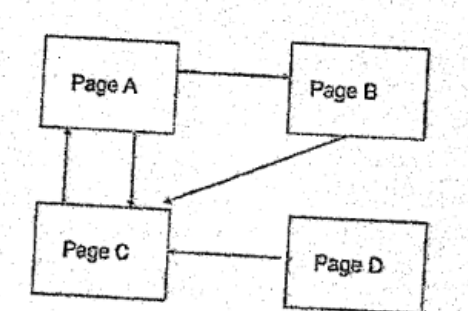
\includegraphics[width=3.2in]{images/dm_76ch_pagerank.png}

      \item Write short notes on: Page Rank algorithm. \hfill [5] (\bo{79 Bh})
        \lb Write short notes on: Page Rank. \hfill [5] (\bo{69 Ch})

      \item Write short notes on: Page rank algorithm in Web mining. \hfill [4] (\bo{78 Bh})

      \item Write short notes on: Web mining. \hfill [4] (73 Shr) [3] (\bo{74 Ch}) [--] (\bo{70 Ch}) [4] (79 Ba)
        \lb Write short notes on: www mining. \hfill [4] (\bo{73 Ch})
    \end{enumerate}

  \subsection{Time-series data mining}
    \begin{enumerate}[topsep=0pt, noitemsep]
      \item Explain Time series data mining in brief. \hfill [6] (72 Ka)

      \item What are the challenges of web mining? Explain about time series data mining with an example. \hfill [5] (\bo{75 Ch})

      \item Explain seasonality in time series data. \hfill [5] (70 Asa)

      \item Write short notes on: Time Series Data Mining. \hfill [5] (80 Ba) [3] (\bo{74 Ch}) [4] (\bo{72 Ch}) [--] (71 Shr) [5] (\bo{82 Bh}) [4] (\bo{81 Bh}) [4] (79 Ba) [4] (\bo{73 Ch})
    \end{enumerate}

\end{document}
